% !TeX spellcheck = cs_CZ
%{\tikzset{external/prefix={tikz/FYZII/}}
% \tikzset{external/figure name/.add={ch20_}{}}
%---------------------------------------------------------------------------------------------------
% file fey2ch20.tex
%---------------------------------------------------------------------------------------------------
%=========================== Kapitola: Řešení Maxwellových rovnic ve volném prostoru  ==============
\chapter{Řešení Maxwellových rovnic ve volném prostoru}\label{fyz:IIchaXX}
\minitoc
  \section{Vlny ve volném prostoru. Rovinné vlny}\label{fyz:IIchaXXsecI}
  \section{Trojrozměrné vlny}\label{fyz:IIchaXXsecII}
  \section{Vědecká obrazotvornost}\label{fyz:IIchaXXsecIII}
  \section{Kulové vlny}\label{fyz:IIchaXXsecIV}
  \section{Příklady a cvičení}\label{fyz:IIchaXXsecV}


    \begin{figure}[ht!] %\ref{fyz_fig643}
      \centering
      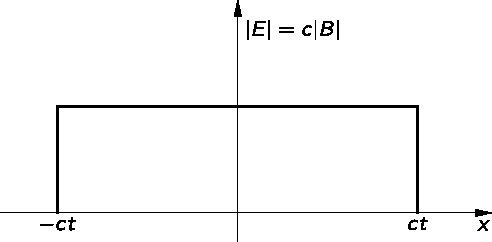
\includegraphics[width=0.7\linewidth]{fyz_fig643.pdf}
      \caption{
               (\cite[s.~707]{Feynman02})}
      \label{fyz_fig643}
    \end{figure}


    \begin{figure}[ht!] %\ref{fyz_fig644}
      \centering
      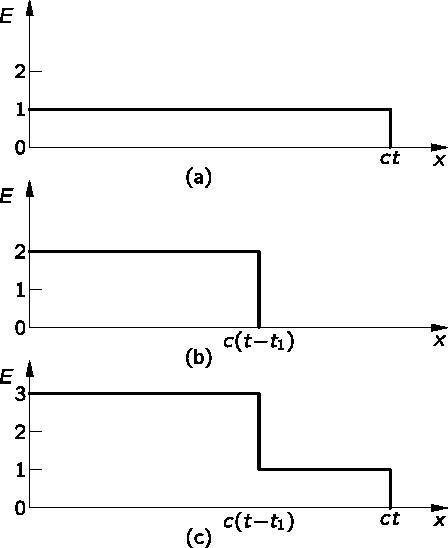
\includegraphics[width=0.7\linewidth]{fyz_fig644.pdf}
      \caption{
               (\cite[s.~707]{Feynman02})}
      \label{fyz_fig644}
    \end{figure}


    \begin{figure}[ht!] %\ref{fyz_fig645}
      \centering
      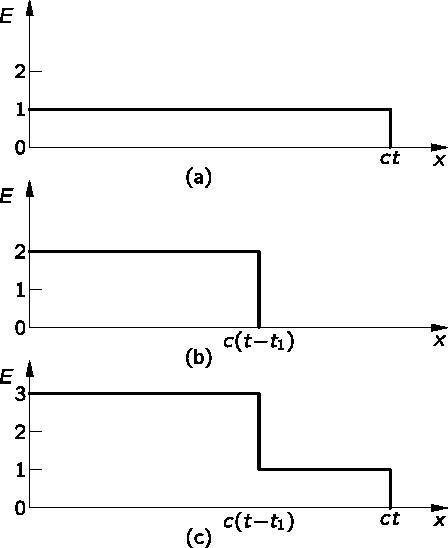
\includegraphics[width=0.7\linewidth]{fyz_fig645.pdf}
      \caption{
               (\cite[s.~707]{Feynman02})}
      \label{fyz_fig645}
    \end{figure}

    \begin{figure}[ht!] %\ref{fyz_fig646}
      \centering
      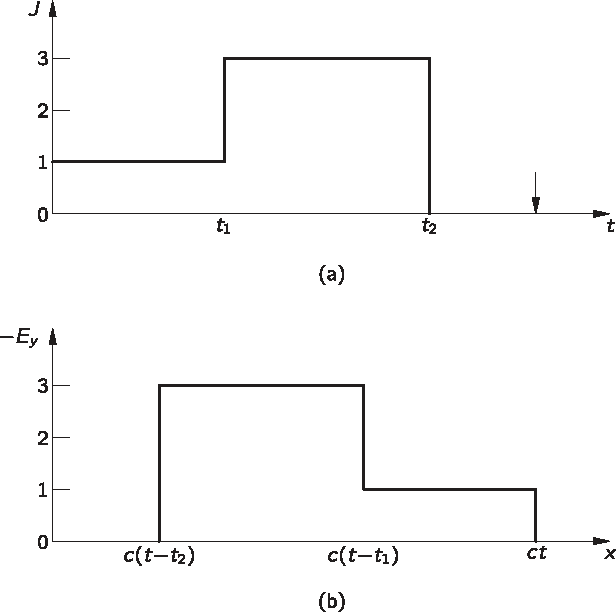
\includegraphics[width=0.7\linewidth]{fyz_fig646.pdf}
      \caption{
               (\cite[s.~707]{Feynman02})}
      \label{fyz_fig646}
    \end{figure}


    \begin{figure}[ht!] %\ref{fyz_fig647}
      \centering
      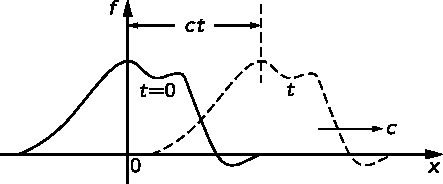
\includegraphics[width=0.7\linewidth]{fyz_fig647.pdf}
      \caption{
               (\cite[s.~707]{Feynman02})}
      \label{fyz_fig647}
    \end{figure}

    \begin{figure}[ht!]
      \centering
      \begin{tabular}{c}
        \subfloat[ ]{\label{fyz_fig649a}
          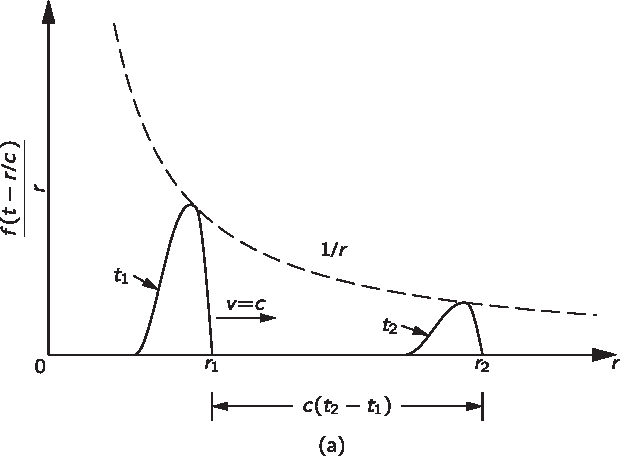
\includegraphics[width=0.7\linewidth]{fyz_fig649a.pdf}}               \\
        \subfloat[ ]{\label{fyz_fig649b}
          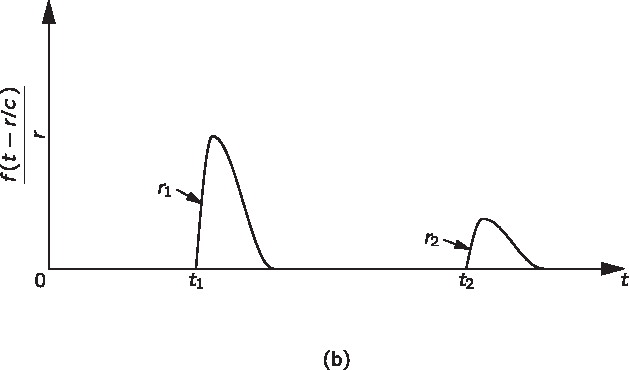
\includegraphics[width=0.7\linewidth]{fyz_fig649b.pdf}}
      \end{tabular}
      \label{fyz_fig649}
      \caption{
               (\cite[s.~748]{Feynman02})}
    \end{figure}
    

%} %tikzset
%---------------------------------------------------------------------------------------------------
%\printbibliography[title={Seznam literatury},heading=subbibliography]
\addcontentsline{toc}{section}{Seznam literatury}